\ifdefined\PROCINCLUDED
%
\else
%%% Please, do not change any of the following parameters.
\documentclass[b5paper,twoside,11pt]{article}
\usepackage[utf8]{inputenc}
\usepackage{geometry}
\voffset=-0.04cm
\headheight=0.6cm
\headsep=0.65cm
\textheight=19.5cm
\footskip=1.25cm
\voffset=-0.04cm
\textwidth=12.6cm
\marginparsep=0cm
\oddsidemargin=0cm
\evensidemargin=0cm
\marginparwidth=0cm
\usepackage{fancyhdr}
\usepackage{url}
\usepackage{graphicx}
\usepackage{mathptmx}
\usepackage{amsmath}
\usepackage{float}
\usepackage{subcaption}
\usepackage{placeins}
\usepackage{gensymb}
\usepackage{enumitem}
\usepackage{blindtext} 
\usepackage{tocloft}
\usepackage[labelsep=period]{caption}
\usepackage{caption}
\usepackage{subcaption}
\captionsetup[table]{skip=7pt}
\captionsetup[figure]{skip=6pt}
\fancyhead{}
\fancyfoot{}
\fancyfoot[LE]{\thepage}
\fancyfoot[RO]{\thepage}
\renewcommand{\headrulewidth}{0.4pt}
\renewcommand{\footrulewidth}{0pt}
\date{}
\def \papertitle#1{\title{#1}}
\pagestyle{fancy}
\def\insertauthor#1#2{
	\begin{minipage}[t]{.45\textwidth}
		\centering
		{\em#1} \\ \vspace*{0.25em}
		#2 \\ \vspace*{1.25em}
	\end{minipage}
}
\def\paperauthors#1{
	\author{
	\begin{minipage}[t]{\textwidth}
	\centering
	#1
	\end{minipage}
	}
}
\def\email#1{\\{\small\protect\url{#1}}}
\def\runningtitle#1{\fancyhead[CO]{\textit{#1}}}
\def\runningauthor#1{\fancyhead[CE]{\textit{#1}}}
\graphicspath{ {figures/} } %%% put all images file into "figures/" subdirectory
\renewcommand{\figurename}{Figure}
\begin{document}
\fi

\papertitle{Procedural fractal plants generation}
\paperauthors{
%%% insert one \insertauthor for each article author, \email part is optional
\insertauthor{Filip Rynkiewicz}{Institute of Information Technology, Lodz University of Technology, ul. Wolczanska 215, 90-924 Lodz, Poland \email{173186@edu.p.lodz.pl}}
\insertauthor{Piotr Napieralski}{Institute of Information Technology, Lodz University of Technology, ul. Wolczanska 215, 90-924 Lodz, Poland}
}
\runningtitle{Lodz University of Technology} %%% brief title for running head
\runningauthor{Rynkiewicz, F. et al.} %%% brief authors for running head


\graphicspath{ {images/} }


\maketitle

%Zrobic zeby to ladnie wszystko przechodzilo jedno z drugiego i nie olewac.

\nocite{*}


\begin{abstract}
Since the beginning of computer era we are trying to imitate nature. The results of those attempts are mathematical equations describing weather, snow flakes, plant growth or influence of species in individual biomes. In computer graphics fractal structure are often used because they can be simple characterize in mathematics. Those forms are common in nature. Self-similar fractals are created in computer graphics using Lindenmayer Systems. This article was formed to analyse efficiency of this algorithm in modelling 3D tree triangle meshes for games. The general motivation of this topic is to produce way to procedural modelling and simplified edition of complicated 3D tree models. By combining L-systems with Bézier curve there is a possibility to produce complicated 3D models. For example tree created with 468 branches having 87200 vertices and it is made in few seconds. In conclusion, time-consuming modelling in 3D programs can be replaced by solution described in this article. 
\end{abstract}

%%% insert your contribution here

\section{Introduction}
Using 3D modelling programs to create a complex 3D mesh of tree is very time consuming, because every branch has to be shaped separately.
To speed up and automatize this process Lindenmayer System can be used. Since 1968, when Aristid Lindenmayer created  grammatic to represent simple multicellular organism, technique has evolved. Now L-Systems are used to manage 3D models of plants\cite{Herbaceus, WebTree, Spray, wlosy, EnviroTree}, fire visualization\cite{Sim}, music\cite{MLSystem} or even neural web\cite{LBrain}. Variaty os usage, flexibility and simplicity of this technique creates a possibility to extend it. Developers over years have used this technique to create software like L-studio\cite{L-Studio}, plugins to 3DsMax to animate plant growth\cite{ABartniak} or in Houdini\cite{LHoud}. \par Most of the algorithms to create 3D tree mesh are generating static models, to change or move branch user must change parameters inside L-System, and recalculate whole model. To prevent unnecessary actions and calculation the \textit{Bézier curve} was added as the tree skeleton. Adding possibility of changing Bézier points along Bézier curve, user can change every branch only by moving it's handler and recalculating only this alternated branch.
\par After long years of plants observations the conclusion was brought, every plant can be treated as a very complex fractal. The most important feature of this structure is self-similarity. In mathematics, a self-similar object is exactly or approximately similar to a part of itself (i.e. the whole has the same shape as one or more of the parts)\cite{SelfSimi}. Because of complexity of plants as fractals the simplifications must be applied. To do this the L-System can be used.
Mentioned above technique is based on rewriting rules, so on replacing sub-terms of a formula with other terms. All formulas and terms are represented as strings, and L-system is all about changing one string to another based on rules. Every system has to have starting word, called axiom, rules of productions and number of iterations, so how many times rules must be applied to word. 

\section{Procedural Systems}
%Co ta so proceduralne systemy. Kazdy podpunkt powinien przechodzic do nastepnego plynnie.
Creating data algorithmically, based on mathematical equations, is the core of procedural system.  This mean that program creates content on its own, or with limited or indirect user input. In case of L-systems there are few possibilities of creating procedural content using simple or more complicated L-systems.

\subsection{OL-system}
Most basic L-System is context-free L-system, called OL-system, where there can be multiple replacement rules to any given value. In example:
\begin{equation}
\begin{aligned}
A \longrightarrow \alpha \\
A \longrightarrow \beta
\end{aligned}
\end{equation}
That means that \textit{A} can be replaced with either $\alpha$ or $\beta$.\\
\par When there is one and only one replacement for the same letter in word, the system is called \textit{DOL-system}, deterministic OL-system.
Giving \textit{axiom}(starting word) as \textit{b}, rules : $b \rightarrow a$ and $a \rightarrow ab$ with 5 iterations simple DOL-system can be created. Example production of this system is shown at \figurename\ref{DOL}.\\
Because L-systems was inspired by nature, usage of it can be found in there. In example  development of cyanobacteria \textit{Anabaena Catenula} can be simulated by DOL-system.
\begin{figure}[!htp]
\centering
  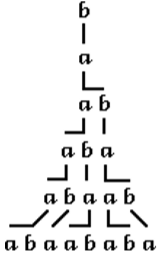
\includegraphics[width=0.15\linewidth]{DOL-system}
\caption{Example of DOL system\cite{prusinABOP} \label{DOL}}
\end{figure}


\subsection{Turtle interpretation of string}
L-systems are operating on symbols, so it's mean that it will always creates list of characters. Every symbol in created word can be classified as \textit{steering character}, in example in Table\ref{steeringTab}.
\begin{table}[!ht]
\caption{Steering characters}\label{steeringTab}
\centering
\begin{tabular}{|l|l|}
\hline
\textbf{sign} & \textbf{discription} \\ 
\hline\hline
+ &Turn  left  by  angle $\delta$. \\ 
- & Turn right by angle  $\delta$ \\ 
\& & Pitch down by angle  $\delta$ \\ 
\string^ & Pitch up by angle  $\delta$ \\ 
\textbackslash & Roll left by angle  $\delta$ \\ 
/ & Roll right by angle  $\delta$ \\ 
\textbar & Turn around, by 180 $\degree $ \\ 
\string[ & Add branch \\ 
\char`\] & End branch \\ 
\string[ A $\ldots$ Z \char`\] & Draw line between points \\
\hline
\end{tabular}
\end{table}

 To create graphical content from it those characters must be parsed to specific action on \textit{turtle}. \textit{Turtle graphics} is term where turtle have it's position, angle which describes the direction in which it is facing and any other parameters that user will use, but position and angle are mandatory. When changing turtle behaviour, so parsing specific character, the different graphical content can be applied. 
\par As it can be seen in the last column in Table\ref{steeringTab} the steering character to draw line between points can be represented by multiple upper cases letters. User can change behaviour of turtle by manipulating those characters. Can be defined which one are representing draw line and which are just to create randomness of given L-system.



\subsection{Bracket L-System}
OL-systems always create one long continued line. To add branching like behaviour, new characters must be added. Using \textit{[} and \textit{]} the \textit{branches} can be created. First character is responsible for starting the branch and next for closing it. Branch is simply new line in geometric interpretation of string created by L-system \figurename\ref{branchingL}.
\begin{figure}[!htp]
\centering
  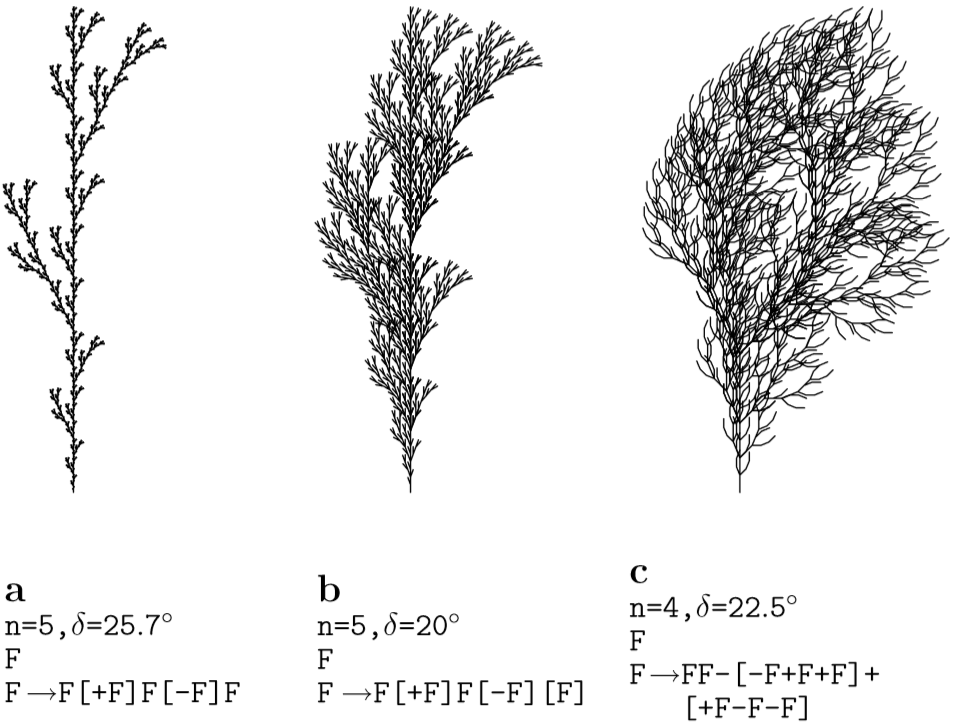
\includegraphics[width=0.7\linewidth]{branchingL}
\caption{Example of Bracket L-system\cite{prusinABOP} \label{branchingL}}
\end{figure}





\subsection{Parametric L-system}
To create more complicated models the parametric L-system was developed. Thanks to parameters L-system can change the values of variables, in example the steering angle of branch. When in OL-system the sign \textit{+} was strictly assigned to hard-coded value, in this approach the value can be changed in every iteration using \textit{+(r)} where \textit{r} is some kind of parameter. Every letter or string must have brackets immediately behind it and within them there can be multiple parameters, separated with comma, also mathematical expressions can be applied between parameters. Example:
\begin{equation}\label{paramEx}
C(x\cdot e,e\backslash 2,a+c,b-d,g)
\end{equation}
As can be seen in Equation~\ref{paramEx} the operands between parameters can be every mathematical operand that can be applied between two floating point numbers.
\section{Bézier curves}
%wprowadzic co to jest krzywa Beziera, dlaczego tego uzywam i po co. Zeby nie bylo z dupy. Dopisac do kazdego co jest co.
Combining all mentioned above L-systems user can create model of plan, but without any possibility to change it without recalculating whole system. To add this feature in this work the Bézier curves was added. It will create whole skeleton of tree, and then based on it the mesh will be created.

Bézier curve is parametric curve, that can be generated under the control of other points. Approximate tangents by using control points are used to generate curve. The Bézier curve can be represented mathematically as
\begin{equation}
\sum\limits_{k=0}^n P_i B_{i}^{n}(t)
\end{equation}
Where $P_i$ is the set of points and $B_{i}^{n}(t)$ represents the Bernstein polynomials which are given by 
\begin{equation}
B_{i}^{n}(t)=\binom{n}{i}(1-t)^{n-i}t^{i}
\end{equation}
Where \textbf{n} is the polynomial degree, \textbf{i} is the index, and \textbf{t} is the variable.
\newline
A B-spline curve is defined as a linear combination of control points $P_i$ and B-spline basis function $N_i	 k (t)$ given by
  \begin{equation}
  C(t)=\sum\limits_{i=0}^n P_i N_{i}^{k}(t)\quad n>=k-1, \quad t \in [tk-1,tn+1]
  \end{equation}
where
\begin{itemize}
\item \begin{equation}\label{conPoi}
P_i={t_0,t_1,\ldots,n},
\end{equation}
$P_i$ describes the control points.
\item $k$ is the order of the polynomial segments of the B-spline curve. Order ${k}$ means that the curve is made up of piecewise polynomial segments of degree $k - 1$.
\item The $Ni,k(t)$ are the “normalized B-spline blending functions”. They are described by the order k and by a non-decreasing sequence of real numbers normally called the “knot sequence”.
\begin{equation}
t_i:i={0,\ldots n+K}
\end{equation}
\end{itemize}
$N_i, k$ functions are described as 
\begin{equation} N_{i}^{1}(t)\;
\begin{cases} 1\qquad \;if \, t_i\leq t< t_{i+1}\:and\: t_i<t_{i+1} \\ 
0 \qquad   Otherwise
 \end{cases}
  \end{equation}
  
  if $k > 1$
   \begin{equation}
  N_{i}^{k}(t)=\frac{t-t_i}{t_{i+k-1}} N_{i}^{k-1}(t) + \frac{t_{i+k} - t}{t_{i+k} - t_{i+1}} N_{i+1}^{k-1}(t)
 \end{equation}
 also
    \begin{equation}
    t\in[t_{k-1},t_{n+1})	
 \end{equation}

\section{Methods}
To implement program, from which screenshot will be presented ,all mentioned above methods was used. Implementation was write in Unity Engine version of C\# called Mono. To do this those custom classes was used:
\begin{itemize}[labelindent=5.5em,labelsep=1cm,leftmargin=*]
\item [LType] description of parameter, its definition as float and name of object
\item [LFunction] definition of production and collection of parameters used in this production
\item [LObject] object of L-System
\item [PosRot] quaternion and position
\end{itemize}
Every \textit{LObject} have list of \textit{LFunction} and Dictionary of \textit{LType}, where \textit{Key} is string name and \textit{Value} is float.
Class where are all methods that calculates L-System productions is \textit{Interpreter}, where there are 2  functions \textit{CreateTreeString and} \textit{CreateBezierTree(LObject currentObject)}. First create word from rules and second creates tree skeleton based on this word. \par
Word is created by replacing one string by another using rules corresponded to LObject. Because in this implementation only Parametric L-system is used, all parameters must be evaluated in every iteration. There are two main cases to do this. When parameters inside bracket have mathematical expression, and when they don't. Second event is simpler to evaluate because algorithm have to find corresponded value to string representation in Dictionary, and than change it for float value. It's performed only at the beginning of algorithm, and with every function. Thanks to this, algorithm does not need to change every parameter in every iteration, it's done only once.
In example Equation~\ref{eq:staticEv}
\begin{equation} \label{eq:staticEv}
!(vr)F(50)[ \&(a)F(50)A]/(d2) \quad\longrightarrow\quad !(2.13)F(50)[ \&(0.45)F(50)A]/(11.3)
 \end{equation}
\newpage
Parameters that have mathematical expression between them have another approach to evaluate them. At first parameters have to be changed to float values then expression must be specified and the last step is to interpret, calculate value as float and then return it as string value.
  %wyjasnic co to jest F(l) i inne literki.
  \begin{equation}\label{eq:dynaEv}
  F(l) \rightarrow F(l \cdot lr)
  \end{equation}
  In this example at Equation~\ref{eq:dynaEv} the rule $F(l)$ must be found in list of production of current \textit{LObject}, \textit{l} and \textit{lr} parameters will have to be found in Dictionary of parameters, $ \cdot$ sign must be interpreted as multiplication sign, and the last step is to return result as string representation of float, so if \textit{l = 6} and \textit{lr = 0.32} the result of this rule would be \textit{F(1.92)}.\par
Second part of algorithm is to generate tree skeleton, based on created before word. String may consist of several thousand characters, so analysing it is the most time consuming part of this algorithm.
Every Bézier Curve has it's parameters such as \textit{normal, bi normal and tangent vector}, corresponded to \textit{X,Y and Z position}. Every branch is separate Bézier Curve, which consist of Bézier Points. Those structures can be moved, deleted or added. That operations are based on steering characters in the word.	
Last step is to generate  mesh based on points of skeleton. Every point on Bézier curve is center of one 3D cylindrical mesh. Normal, binormal and tangend are used in this part to calculate properly bending angles.
All calculation are based on Quaternions rotations, to ensure appropriate angles, and because that how the Unity is handling the angles.
\begin{figure}[!htp]
\centering
  \includegraphics[width=1\linewidth]{diagram2}
\caption{Flow chart of this algorithm \label{diagram}}
\end{figure}


\iffalse
\begin{figure}[!htbp] 

\begin{subfigure}{.5\textwidth}  
 \centering   
 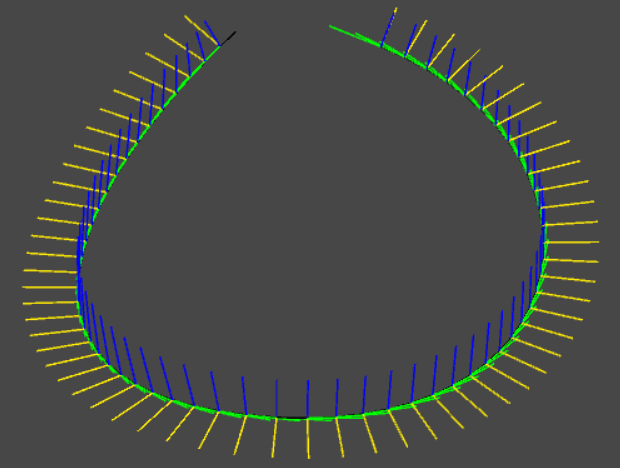
\includegraphics[width=1.0\linewidth]
 {drawDirection} \caption{Visualisation of direction(green), normal and binormal (yellow) of splain.   \label{unity.drawDirection}} 
\end{subfigure} 
\begin{subfigure}{.5\textwidth}  
 \centering  
  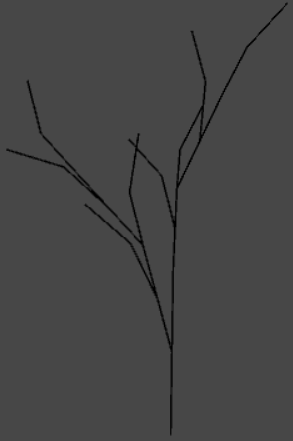
\includegraphics[width=0.5\linewidth]{krzyweDrzewo} 
  \caption{Tree skeleton. \label{unity.krzyweDrzewo}} 
  \end{subfigure}
  \begin{subfigure}{.5\textwidth}
     \centering   
     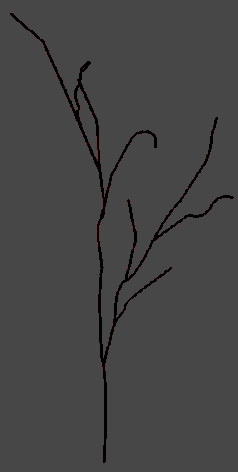
\includegraphics[width=0.5\linewidth]{krzyweDrzewoMod} 
     \caption{Tree skeleton after modyfication. \label{unity.krzyweDrzewoMod}} 
   \end{subfigure}
\begin{subfigure}{.5\textwidth} \ContinuedFloat
  \centering  
  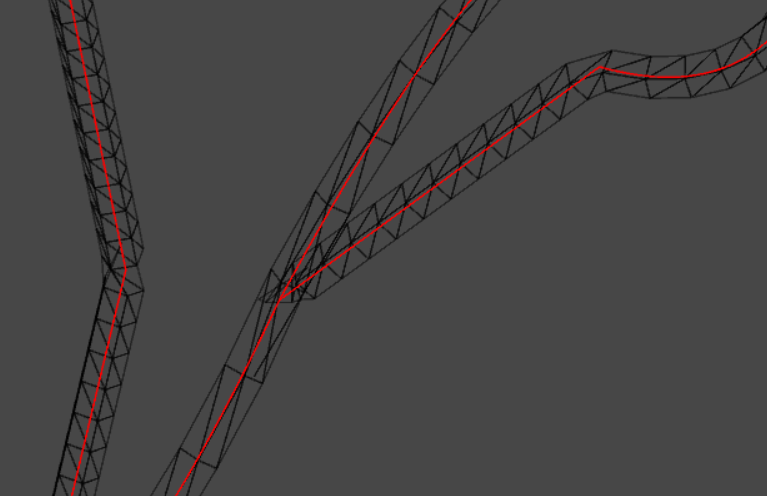
\includegraphics[width=1.0\linewidth]{krzyweDrzewoSiatka2} 
  \caption{Mesh on skeleton after modyfication. \label{unity.krzyweDrzewoSiatka}}
\end{subfigure} 
       \caption{ddd} \label{unity.direction} 
       \end{figure}
   \fi
\section{Results}
For each of the example the same values was used. Five segments on the side surface and five points on spline, it's mean that every curve was divided on five equal parts. Each result of implemented algorithm was divided into two pictures, screenshot of model generated by algorithm and model after changes. Changes was made by transforming Bézier Points on corresponded to branch Bézier Curve. First all the example and it's description was shown, then the pictures. Description of every example System contains rules, axiom and number of iteration used within it.
\subsection*{Example 1}
In first example for 5 iterations the number of branches is 468, word forming tree have 46086 chars and number of vertices in model is 87200.\par
This example is modification of simple fractal plant described in \cite{prusinABOP}.
Every branch is directed at 25  $\degree$ relative to parent branch. As it can be seen at the \figurename \ref{przyklad1.siatka}, the model created by algorithm is complex, using only two rule and one variable. Model after changes have been shown at  \figurename \ref{przyklad1.siatkaMOD}. Every branch in tree have been altered according to user actions.\par 
Rules: \newline
\begin{equation}
F(l)\rightarrow F(l\cdot2) 
\end{equation}
\begin{equation}
X(l) \rightarrow F(l)[/(r)X(l)]F(l)[\setminus(r)X(l)-(r)X(l)]F(l)[\setminus(r)X(l)+(r)X(l)] 
\end{equation}
Axiom:
\begin{center}
X(1)
\end{center}
Number of iterations:
\begin{center}
4
\end{center}
Variables:
\begin{equation}
r\rightarrow 25
\end{equation}


\FloatBarrier
%~~~~~~~~~~~~~~~~~~~~~~~~~~~~~~~~~~
\begin{figure}[!htp]

\centering
\begin{subfigure}{.49\textwidth}
  \centering
  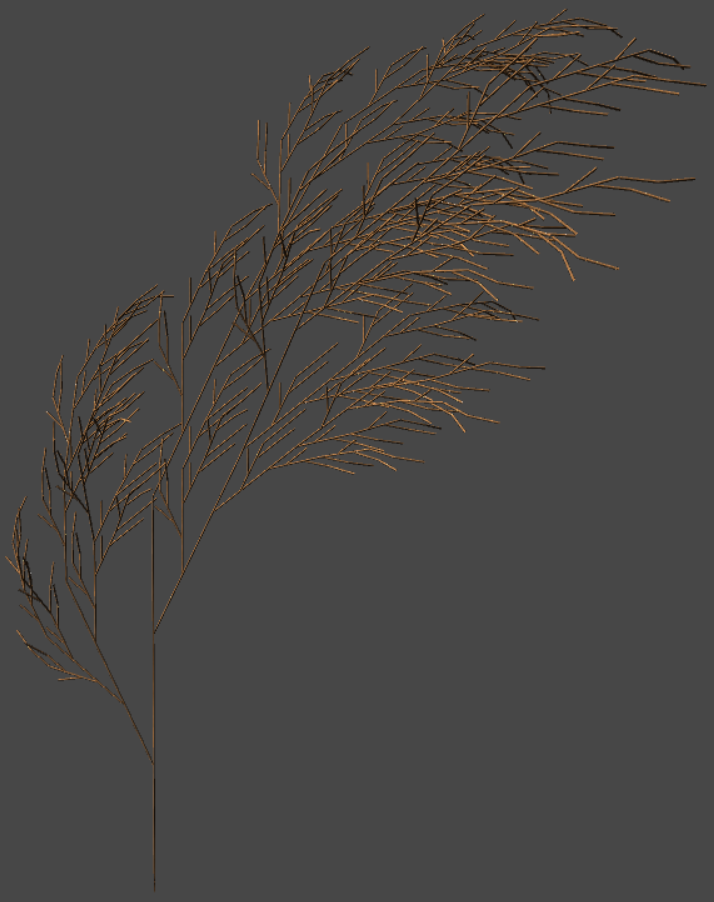
\includegraphics[width=0.8\linewidth]{siatka1}
\caption{Mesh without modification.\\Own source. \label{przyklad1.siatka}}
\end{subfigure}
%\\
\begin{subfigure}{.49\textwidth}
  \centering
  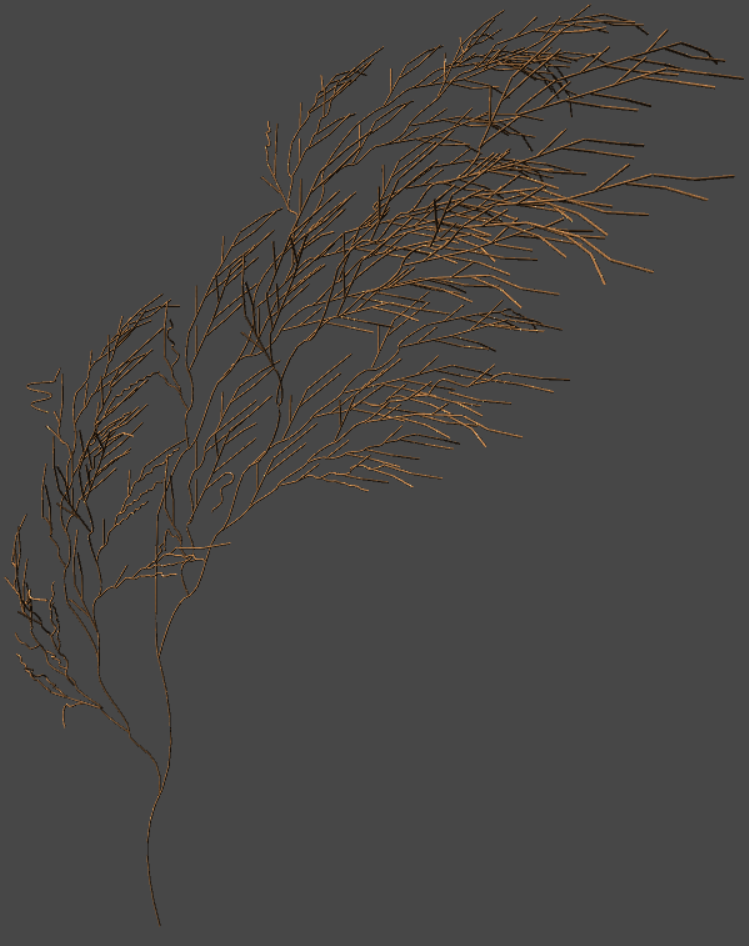
\includegraphics[width=0.8\linewidth]{siatkaMOD1}
\caption{Mesh after modification.\\Own source. \label{przyklad1.siatkaMOD}}
\end{subfigure}
\caption{Comparison of meshes for example  1.}
\label{przyklad1}
\end{figure}
%~~~~~~~~~~~~~~~~~~~~~~~~~~~~~~~~~~
\newpage
%dodac refleksje i po co to w ogole robie.
\subsection*{Example 2}
Next example have 171 branches, world forming tree have 24918 chars and 73700 vertices in model.\par
In this case the custom and longer rules have been used to make model looks like non-deterministic and more chaotic. Model before changes was shown at \figurename\ref{przyklad2.siatka}, and after changes at \figurename\ref{przyklad2.siatkaMOD}. In first example every variable had exactly one parameter without any mathematical operations, except $F(l \cdot 2)$. But in the second  every operation on parameter had to be evaluated and changed to float value, so the time of the calculation had increased significantly. Thanks to usage of multiple parameters and operation between them user can create more complicated structures, using less rules, but for the price of time for parameter evaluations.\\
Rules: \newline
\begin{equation}
F(l)\rightarrow F(l\cdot2) 
\end{equation}
\begin{equation}
X(l,w) \rightarrow F(w\cdot l)[/(r\cdot l)X(l,w)-(r)X(w,w)]+(r)F(l)[\setminus(l)X(l,w)+(r)X(l,w)]-(r)F(w)
\end{equation}
Axiom:
\begin{center}
X(1)
\end{center}
Number of iterations:
\begin{center}
5
\end{center}
Variables:
\begin{equation}
r\rightarrow 17.2
\end{equation}

\begin{figure}[!htp]
\centering
\begin{subfigure}{.49\textwidth}
  \centering
  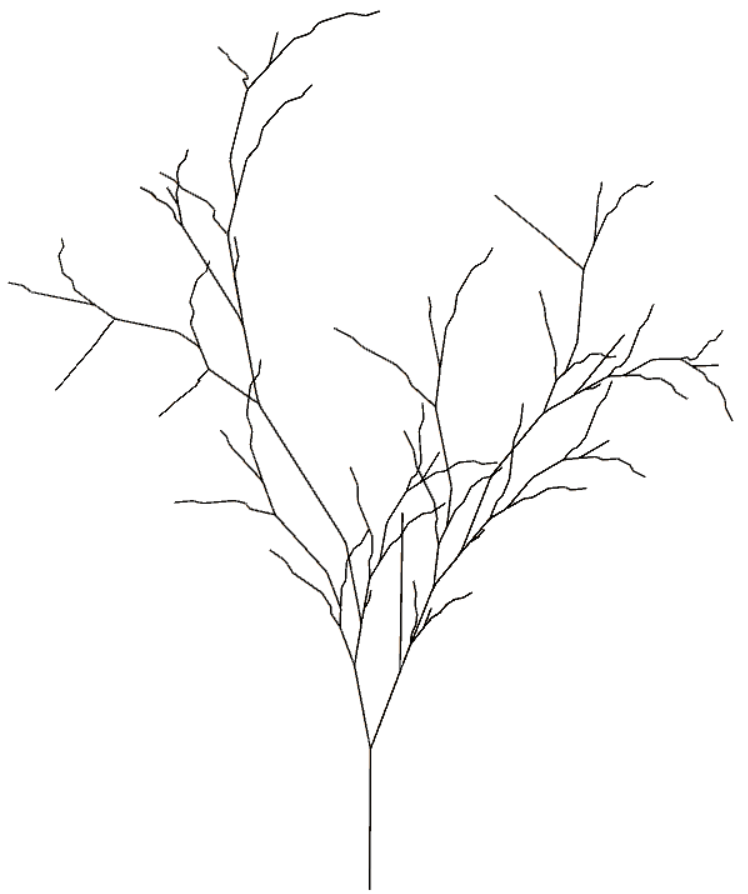
\includegraphics[width=0.8\linewidth]{przyklad2}
\caption{Mesh withouth modification.\\Own source. \label{przyklad2.siatka}}
\end{subfigure}
\begin{subfigure}{.49\textwidth}
  \centering
  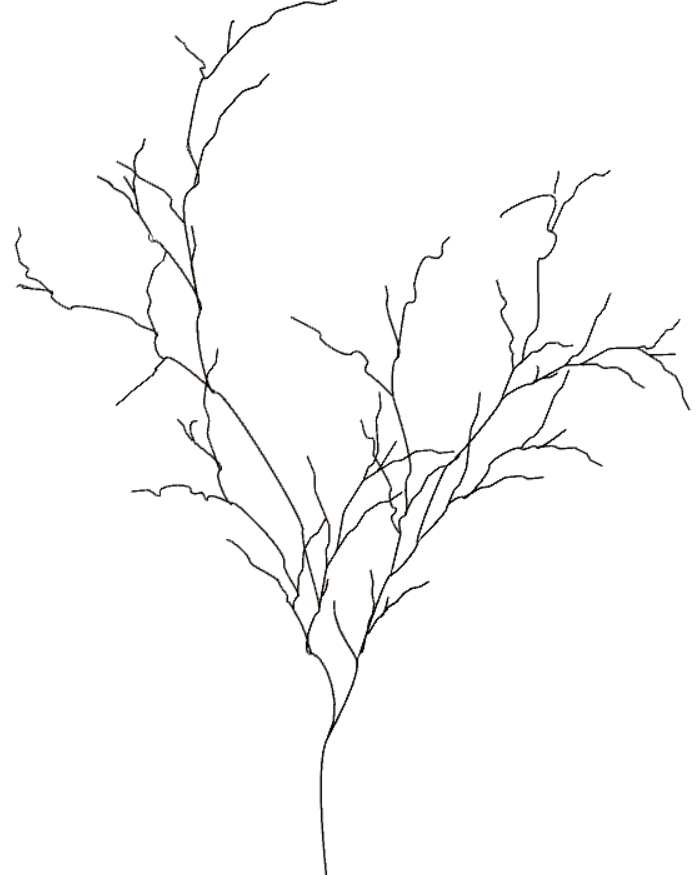
\includegraphics[width=0.8\linewidth]{przyklad2MOD}
\caption{Mesh after modification.\\Own source. \label{przyklad2.siatkaMOD}}
\end{subfigure}
\caption{Comparison of meshes for example  2.}
\label{przyklad2}
\end{figure}
\newpage

\subsection*{Example 3}
Last example have 214 branches, world world forming tree have 24918 chars and 73700 vertices in model. 
\figurename \ref{przyklad3.siatka} presents unchanged model of last example, \figurename \ref{przyklad3.siatkaMOD} same model after changes. Creating more complicated rule, based on those in example 2, and adding two more simple rules the model in example 3 is more non-deterministic and tree-like than other examples.
Rules: \newline
\begin{equation}
F(l)\rightarrow F(l\cdot2) 
\end{equation}
\begin{multline*}
X(l,w) \rightarrow F(w\cdot l)[/(r\cdot l)X(l,w)-(r)X(w,w)C(l)]\\
+(r)F(l)[G(l)\setminus(l)X(l,w)+(r)X(l,w)]-(r)F(w)-(r)F(w)
\end{multline*}
\begin{equation}
G(l) \rightarrow F(l/5)[X(l,l)+(r\cdot k)]
\end{equation}
\begin{equation}
C(l) \rightarrow F(l/5)[X(l,l)/(r\cdot k)]
\end{equation}
Axiom:
\begin{center}
X(1,2)
\end{center}
Number of iterations:
\begin{center}
5
\end{center}
Variables:
\begin{equation}
r\rightarrow 23.5
\end{equation}
\begin{equation}
k\rightarrow 0.707
\end{equation}





%~~~~~~~~~~~~~~~~~~~~~~~~~~~~~~~~~~
\begin{figure}[!htp]
\centering
\begin{subfigure}{.49\textwidth}
  \centering
  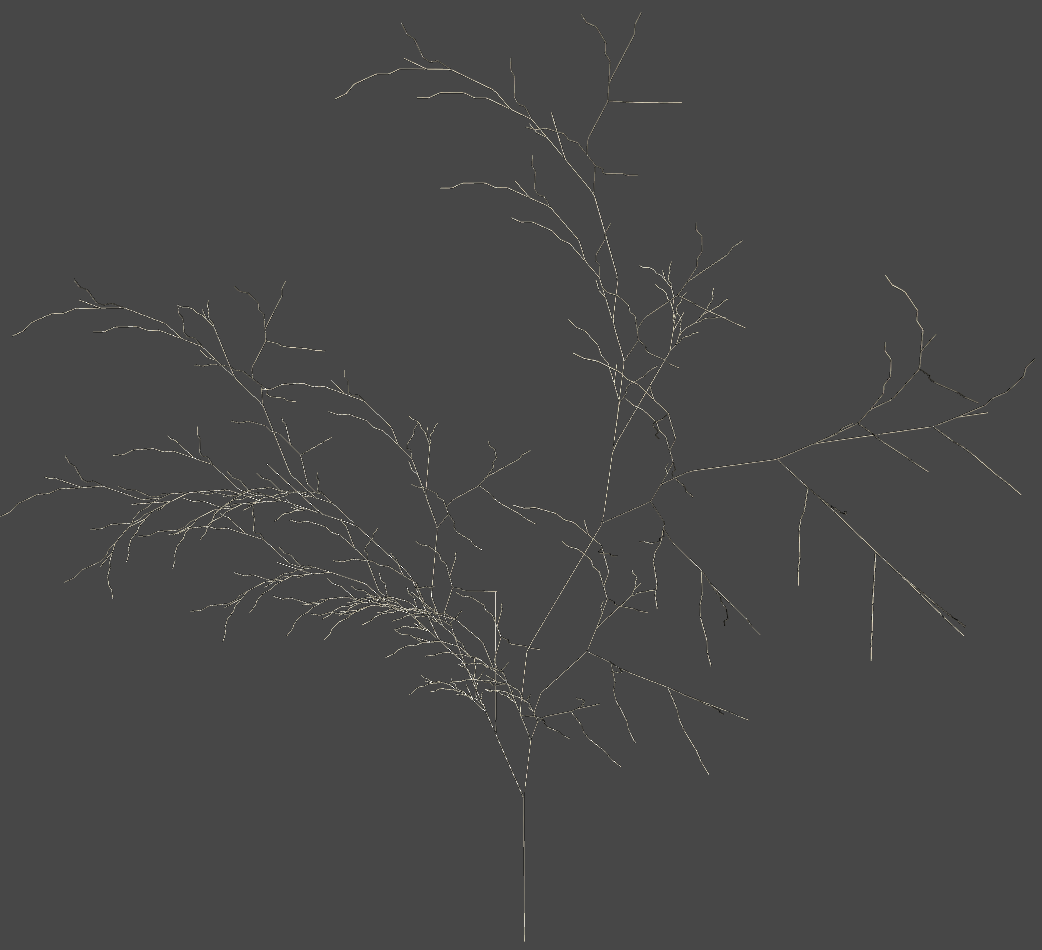
\includegraphics[width=0.8\linewidth]{przyklad3MOD}
\caption{Mesh without modification.\\Own source. \label{przyklad3.siatka}}
\end{subfigure}
%
\begin{subfigure}{.49\textwidth}
  \centering
  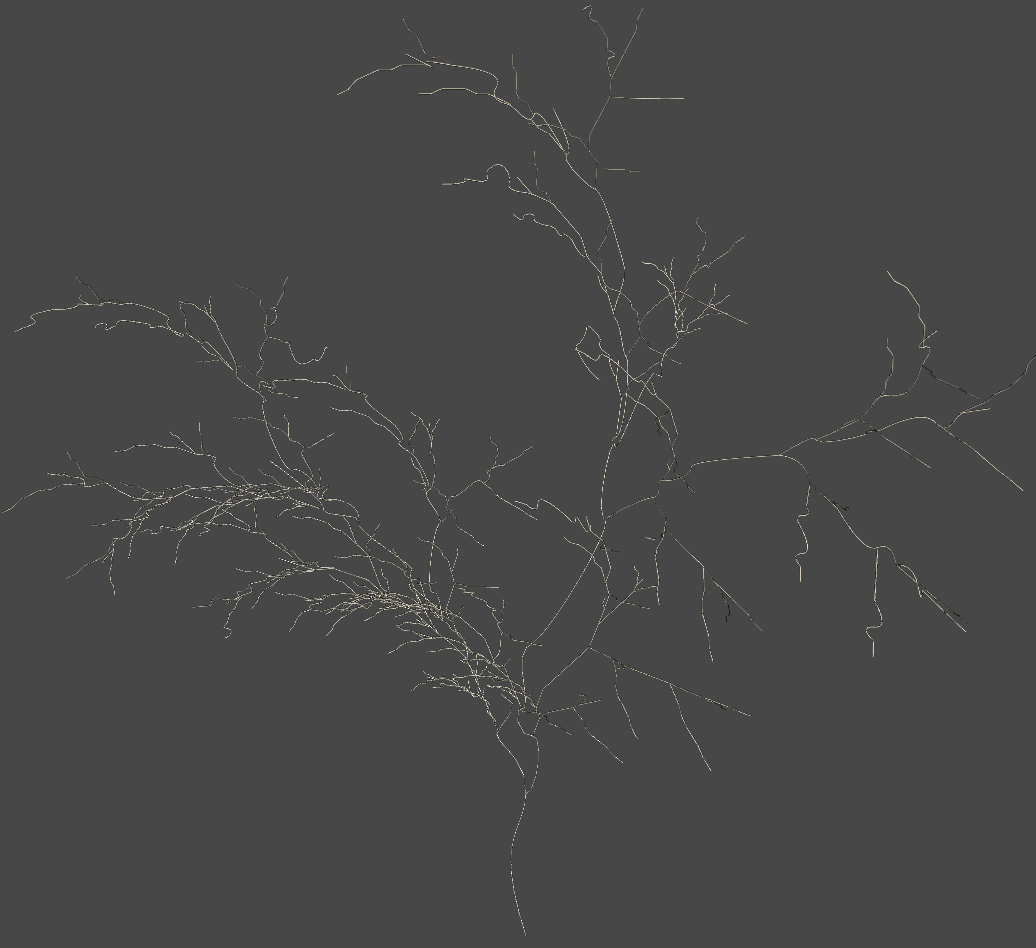
\includegraphics[width=0.8\linewidth]{przyklad3}
\caption{Mesh after modification.\\Own source. \label{przyklad3.siatkaMOD}}
\end{subfigure}
\caption{Comparison of meshes for example  3.}
\label{przyklad3}
\end{figure}
\newpage





\section{Conclusion}
By using technique described before the user can simply generate tree-like model in short time, small amount of vertices, and with ability to change every point of model using Bézier handles. Creating model with 300 branches using normal 3d  software would be very time consuming.We can move our work to machine and automatize process of modelling, using simple parametrized mathematical equations, without even knowing how the modelling software works. And we can do this inside game engine, without other programs.

To evaluate all string into float values the simple parser have been created.
Parser created with this implementation is simple, but creating possibility to evaluate more than 3 parameters, and operations between them, using approaches from this implementation would be very difficult. To ensure that every parameter would be evaluated properly whole implementation will be rewritten into new \textit{Boost Spirit X3} C++ library, and created as \textit{Dynamic-Link Library}. Unity,Unreal Engine and others game engines have ability to write plugins based on \textit{DLL} written in \textbf{C++}, so every engine could have their own implementation of this algorithm.
% use section* for acknowledgement

%Jeszcze raz sprawdz bibliografie
\begin{thebibliography}{99}
\small
\bibitem{Herbaceus}Prusinkiewicz P., Lindenmayer A.,Hanan J.,\textit{ Development models of herbaceous plants for computer imagery purposes},  SIGGRAPH Comput. Graph., New York, 1998
\bibitem{Sim} Zaniewski T., Bangay S., \textit{ Simulation and visualization of fire using extended lindenmayer systems}, AFRIGRAPH '03, Cape Town, 2003
\bibitem{WebTree}Qi H.,Qiu R.,Jia J., \textit{L-system based interactive and lightweight web3D tree modeling}, VRCAI '11, Hong Kong, 2011
\bibitem{EnviroTree}  Zhuming L., and King S., \textit{Simulating tree growth based on internal and environmental factors}, GRAPHITE '05, Dunedin, 2005
\bibitem{Spray}Hanan J., Renton M., Yorston E., \textit{Simulating and visualising spray deposition on plant canopies}, GRAPHITE '03, Melbourne, 2003
\bibitem{MLSystem}Manousakis S., \textit{Musical L-Systems}, The Royal Conservatory,Hague, 2006
\bibitem{LBrain}Palmer M., \textit{Evolved neurogenesis and synaptogenesis for robotic control: the L-brain model}, GECCO '11, Dublin, 2011
\bibitem{L-Studio}L-studio, \url{http://algorithmicbotany.org/virtual_laboratory/}
\bibitem{ABartniak}Bartniak A., \textit{3D animation of plant development using L-systems}, M.Sc. thesis, Lodz, 2013
\bibitem{SelfSimi}Mandelbrot, B., \textit{How long is the coast of Britain? Statistical self-similarity and fractional dimension}, Science, vol. 156, no. 3775, 1967, pp. 636–638. http://www.jstor.org/stable/1721427.
\bibitem{LHoud}Houdini Engine L-System, \url{https://www.sidefx.com/docs/houdini/nodes/sop/lsystem}
\bibitem{prusinABOP}
Prusinkiewicz P., Lindermayer A., \textit{The Algorithmic Beauty of Plants}, Springer , 2004
\bibitem{BSpline}
Bézier curve, \url {http://mathworld.wolfram.com/B-Spline.html}
\bibitem{wlosy}
Fuhrer M. Hairs, \textit{Textures, and Shades: Improving the Realism of Plant Models Generated with L-systems}, M.Sc. thesis, University of Calgary, 2005
\bibitem {LMat} Rozenberg G., Salomaa A. \textit{The mathematical theory of L systems}, Academic Press, New York, 1980

\end{thebibliography}

\ifdefined\PROCINCLUDED
%
\else
\end{document}
\fi
